%\documentclass[12pt, oneside]{article} 
\documentclass[xetex,14pt,serif,compress,hyperref={xetex}]{beamer}
%\documentclass[xetex,14pt,mathserif,serif]{beamer}
%\documentclass[12pt,compress,hyperref={xetex}]{beamer}
%\usepackage[xetex, a4paper, left=2cm, right=2cm, top=2cm,bottom=2cm]{geometry}
\usepackage[cm-default]{fontspec}
\usepackage{xunicode}
\usepackage{xltxtra}
\usetheme{Warsaw}

%\tolerance=1000
%\emergencystretch=0.74cm 

\usepackage{polyglossia}
\setdefaultlanguage[spelling=modern]{russian}
\setotherlanguage{english} 
\defaultfontfeatures{Scale=MatchLowercase}  %% устанавливает поведение шрифтов по умолчанию  
\newfontfamily\cyrillicfont{Linux Libertine} 
\setromanfont[Mapping=tex-text]{Linux Libertine}
\setsansfont[Mapping=tex-text]{Linux Biolinum}
\setmonofont{DejaVu Sans Mono}
%\newfontfamily\cyrillicfont{Liberation Mono} 


%\oddsidemargin=-0.4mm 
%\textwidth=160mm 
%\topmargin=4.6mm 
%\textheight=210mm 
%\parindent=17pt 
%\parskip=3pt

\author{С.~А.~Барвенов, А.~А.~Станкевич}
\title{Git и github в преподавании}
\date{13 мая 2015}
\begin{document}
\begin{frame}
\titlepage
\end{frame}
\begin{frame}{Зачем это нужно?}

\parbox{\linewidth}{\Large{При преподавании «программистcких» курсов 
преподавателю нужно проверять 
исходные коды программы и взаимодействовать со студентами.}}


\end{frame}
\begin{frame}
\parbox{\linewidth}{\Large{Системы контроля версий и облачные сервисы позволяют 
организовать эту работу более системно.}}
\end{frame}
\begin{frame}
\begin{block}{Исторический факт:}
  Одна из первых систем контроля версий (CVS) была создана в 
педагогической практике.
\end{block}
\end{frame}
\begin{frame}{Почему git?}
 \begin{itemize}
  \item Одна из самых распространённых СКВ
  \item Свободная и бесплатная
  \item Кроссплатформенная
  \item Много материалов, в том числе на русском языке
  \item Github работает с гитом, а github самый крупный сервис такого рода
  \item Просто в силу случайных причин ☺
 \end{itemize}

\end{frame}
\begin{frame}{Что даёт получившаяся связка?}
 \begin{itemize}
  \item публиковать в сети задания и оценки;

\item просматривать студенческие листинги, контролируя время их размещения и 
авторство;

\item устанавливать dead-line, т.е. запрещать с определенного момента запись 
работ;

 \end{itemize}

\end{frame}
\begin{frame}{Что даёт получившаяся связка?}
 \begin{itemize}
\item создавать комментарии не только в целом к проекту, но и к определенным 
строкам программы. Указывать на недочёты в проделанной работе и размещать 
указания к выполнению заданий;

\item студенты могут автоматически получать  уведомления о проверке 
работы и 
комментарии преподавателя.
 \end{itemize}

\end{frame}


\begin{frame}{Работа с гитом}
\begin{center}
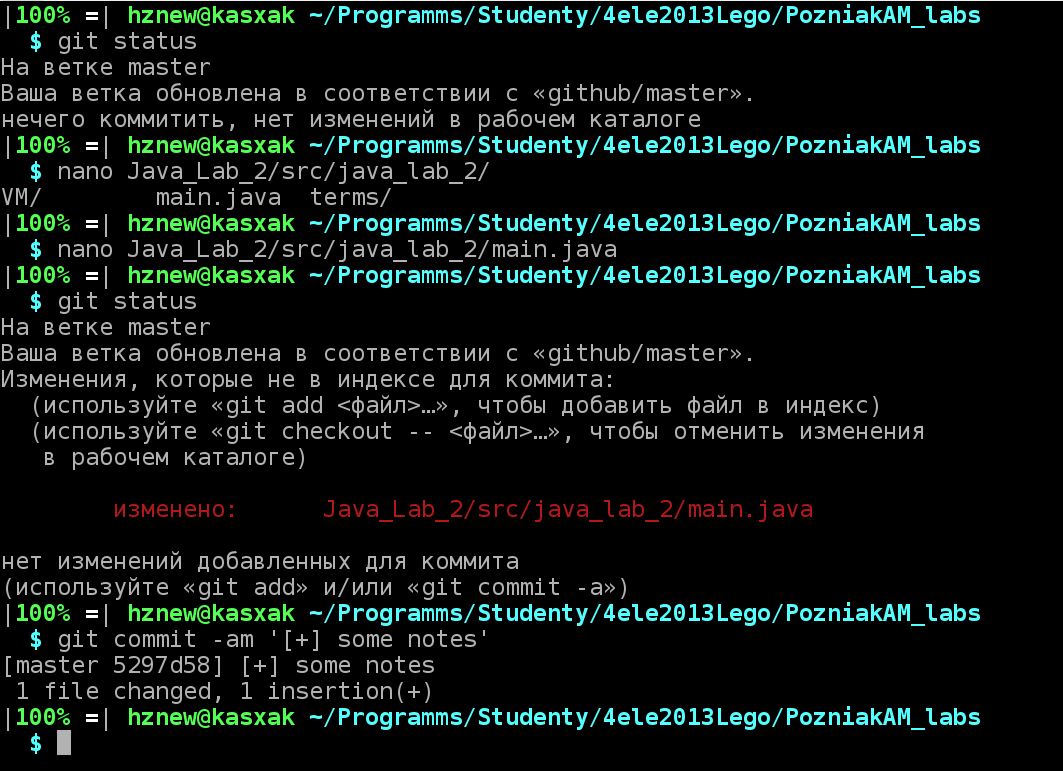
\includegraphics[scale=0.5,keepaspectratio]{snp37.png}
\end{center}
\end{frame}

\begin{frame}{Студенческая группа}
\begin{center}
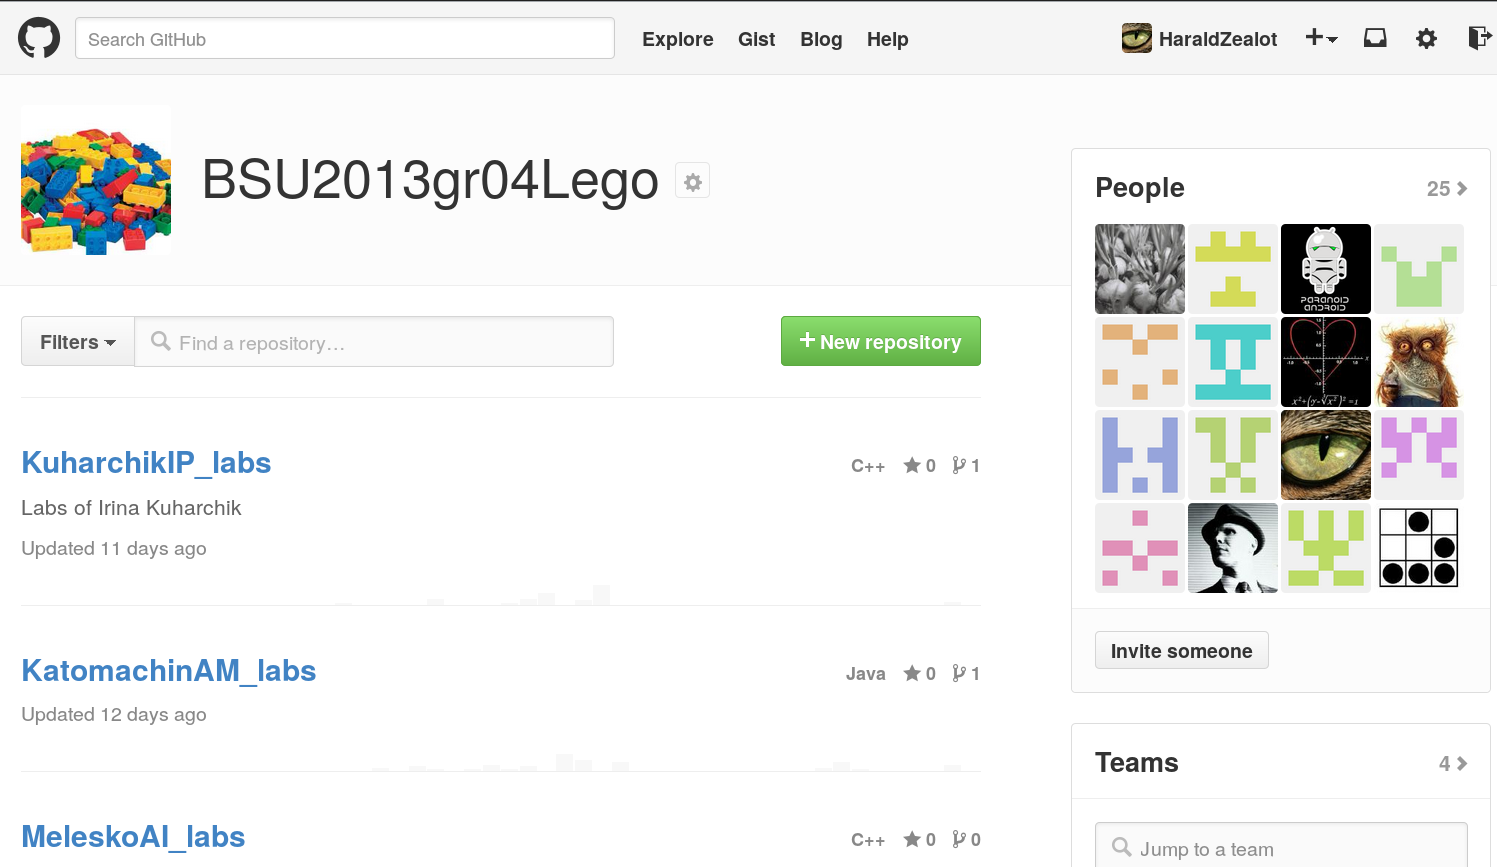
\includegraphics[scale=0.4,keepaspectratio]{snp39.png}
\end{center}
\end{frame}

\begin{frame}{Команда студентов}
\begin{center}
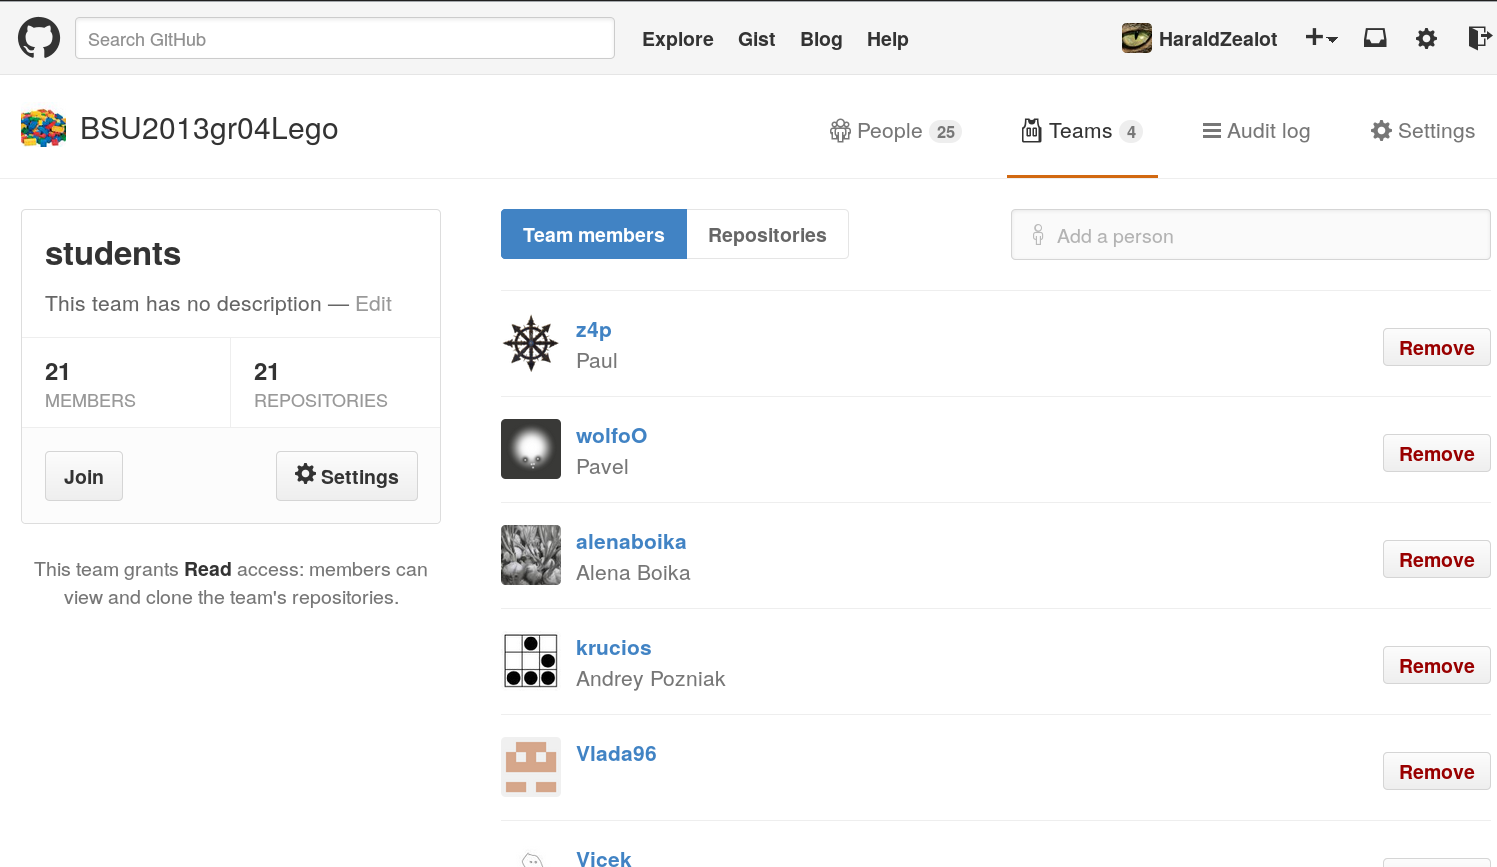
\includegraphics[scale=0.4,keepaspectratio]{snp40.png}
\end{center}
\end{frame}

\begin{frame}{Новости в организации}
\begin{center}

\includegraphics[scale=0.4,keepaspectratio]{snp38.png}
\end{center}
\end{frame}


\begin{frame}{Оценки}
\begin{center}
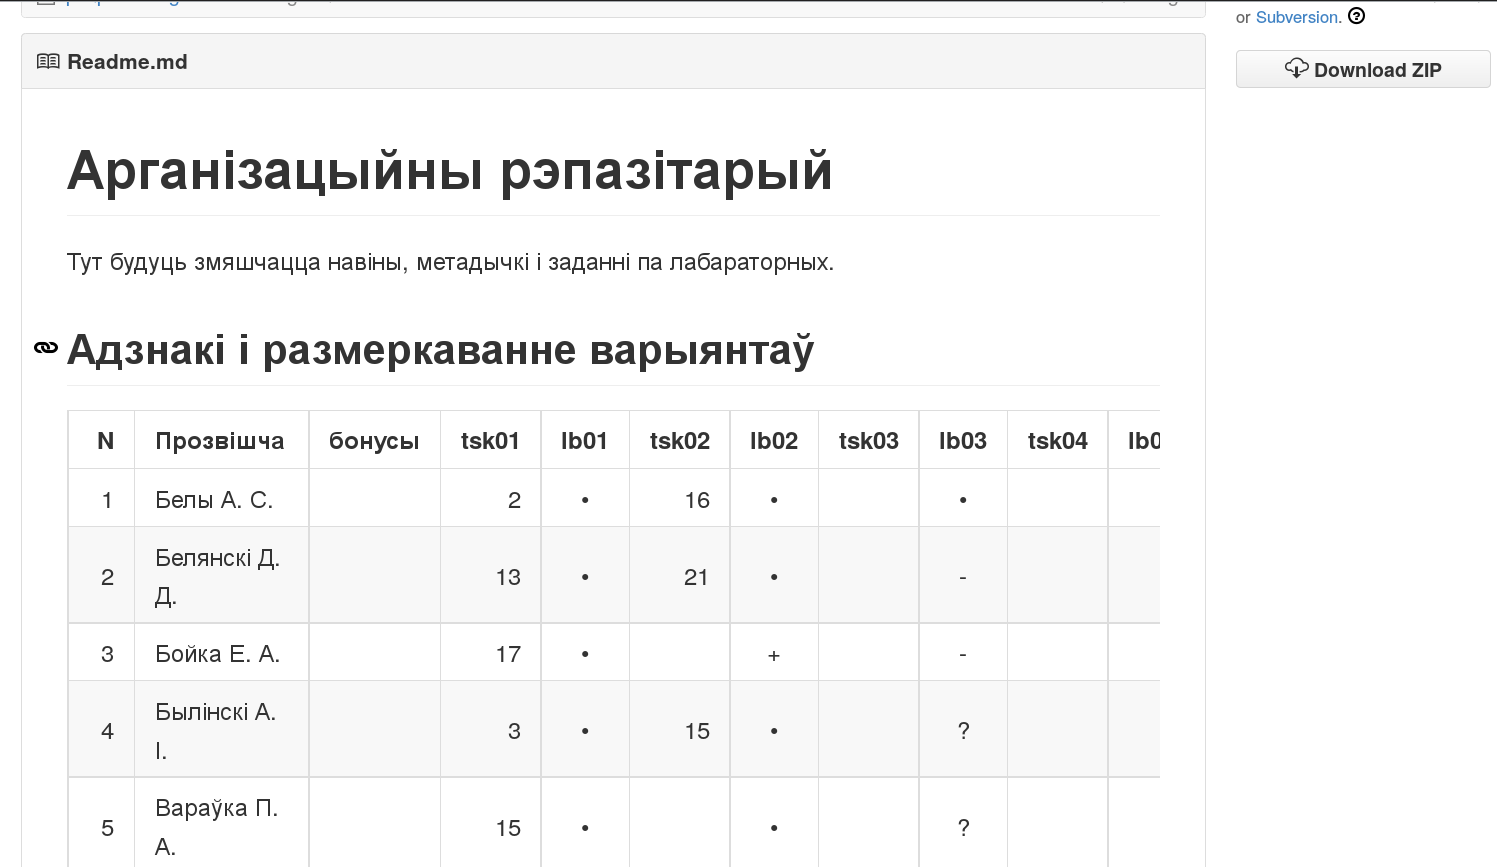
\includegraphics[scale=0.4,keepaspectratio]{snp41.png}
\end{center}
\end{frame}

\begin{frame}{История коммитов}
\begin{center}
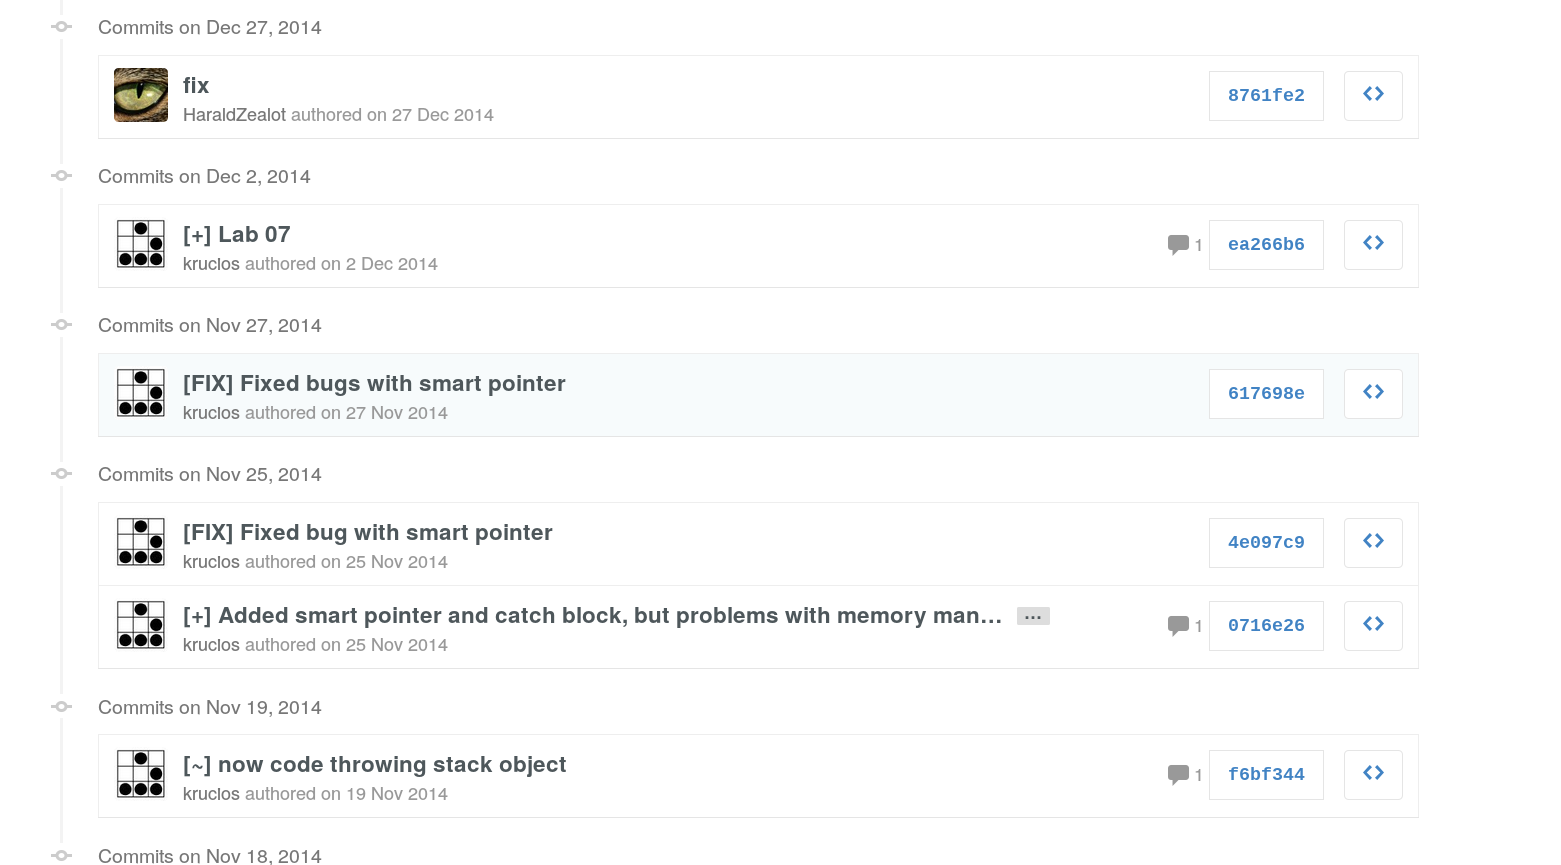
\includegraphics[scale=0.4,keepaspectratio]{snp46.png}
\end{center}
\end{frame}

\begin{frame}{Просмотр изменений}
\begin{center}
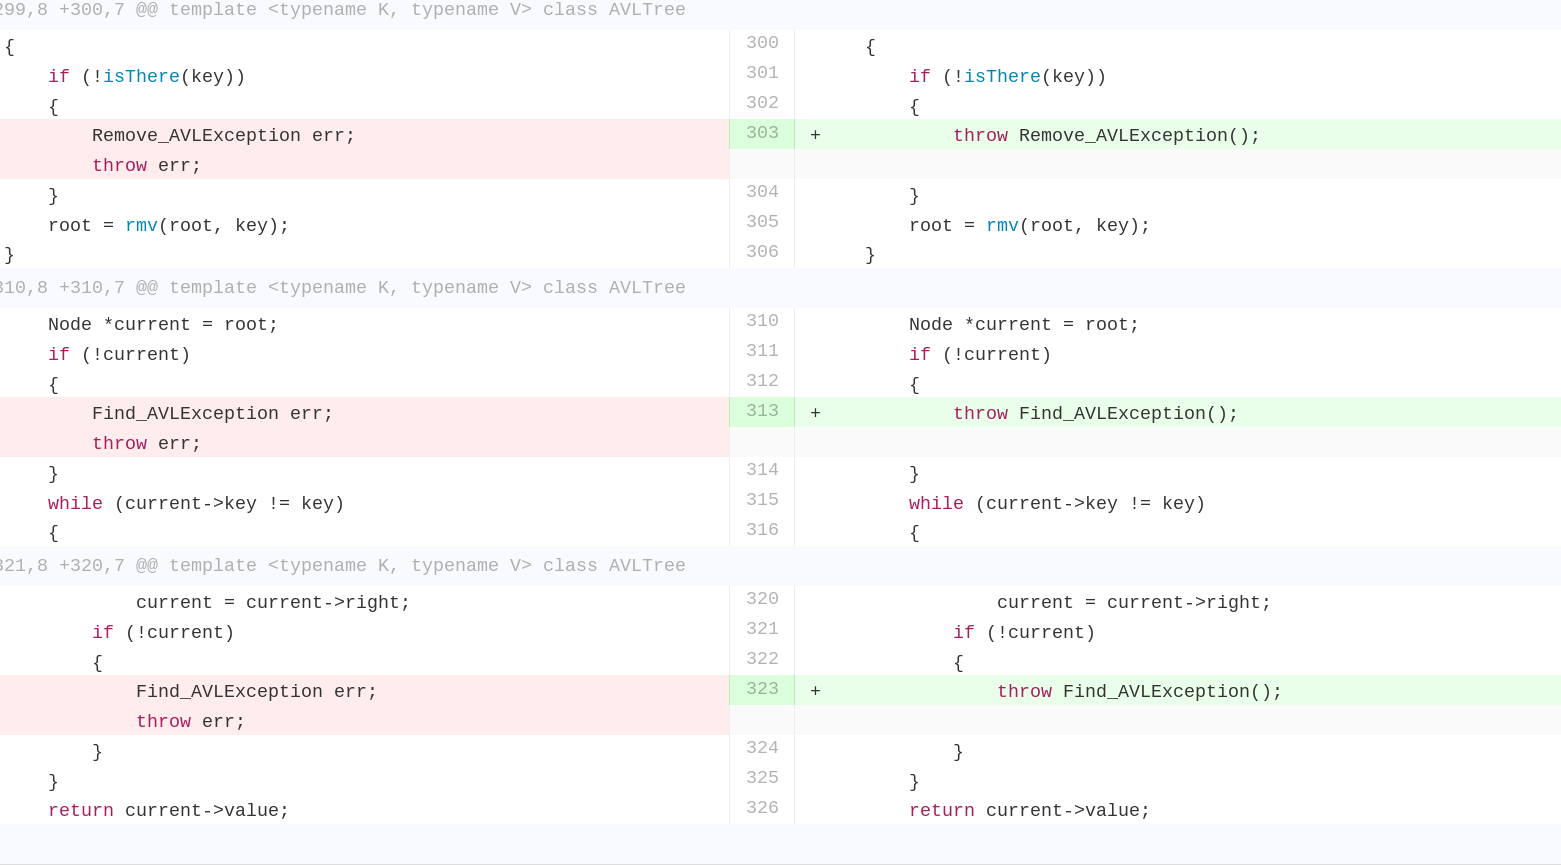
\includegraphics[scale=0.4,keepaspectratio]{snp47.png}
\end{center}
\end{frame}

\begin{frame}{Комментарии к коду}
\begin{center}
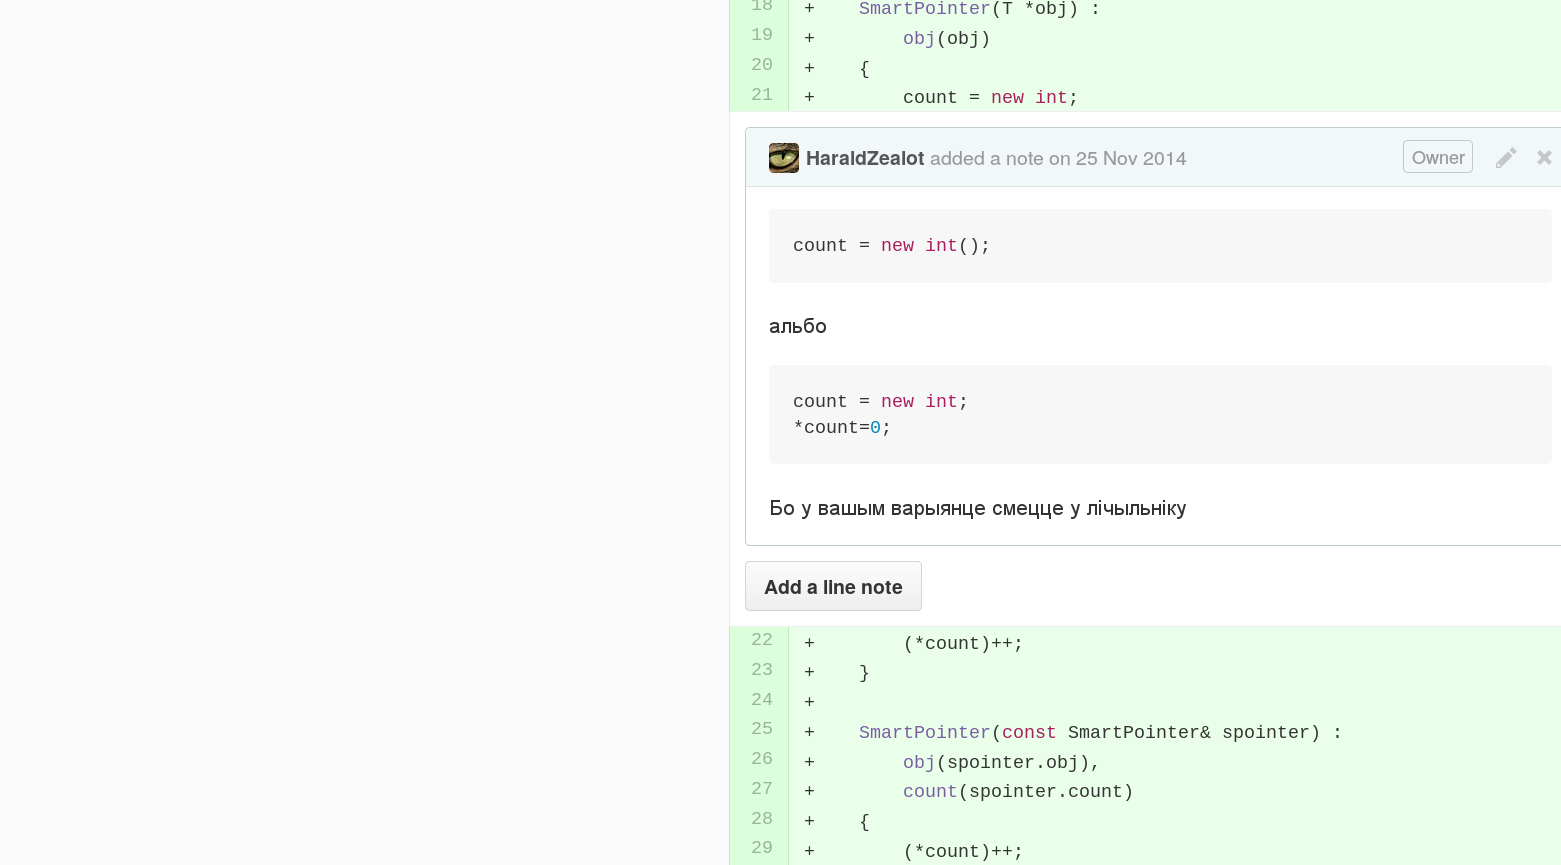
\includegraphics[scale=0.4,keepaspectratio]{snp48.png}
\end{center}
\end{frame}


\begin{frame}{Указания на исправление бага}
\begin{center}
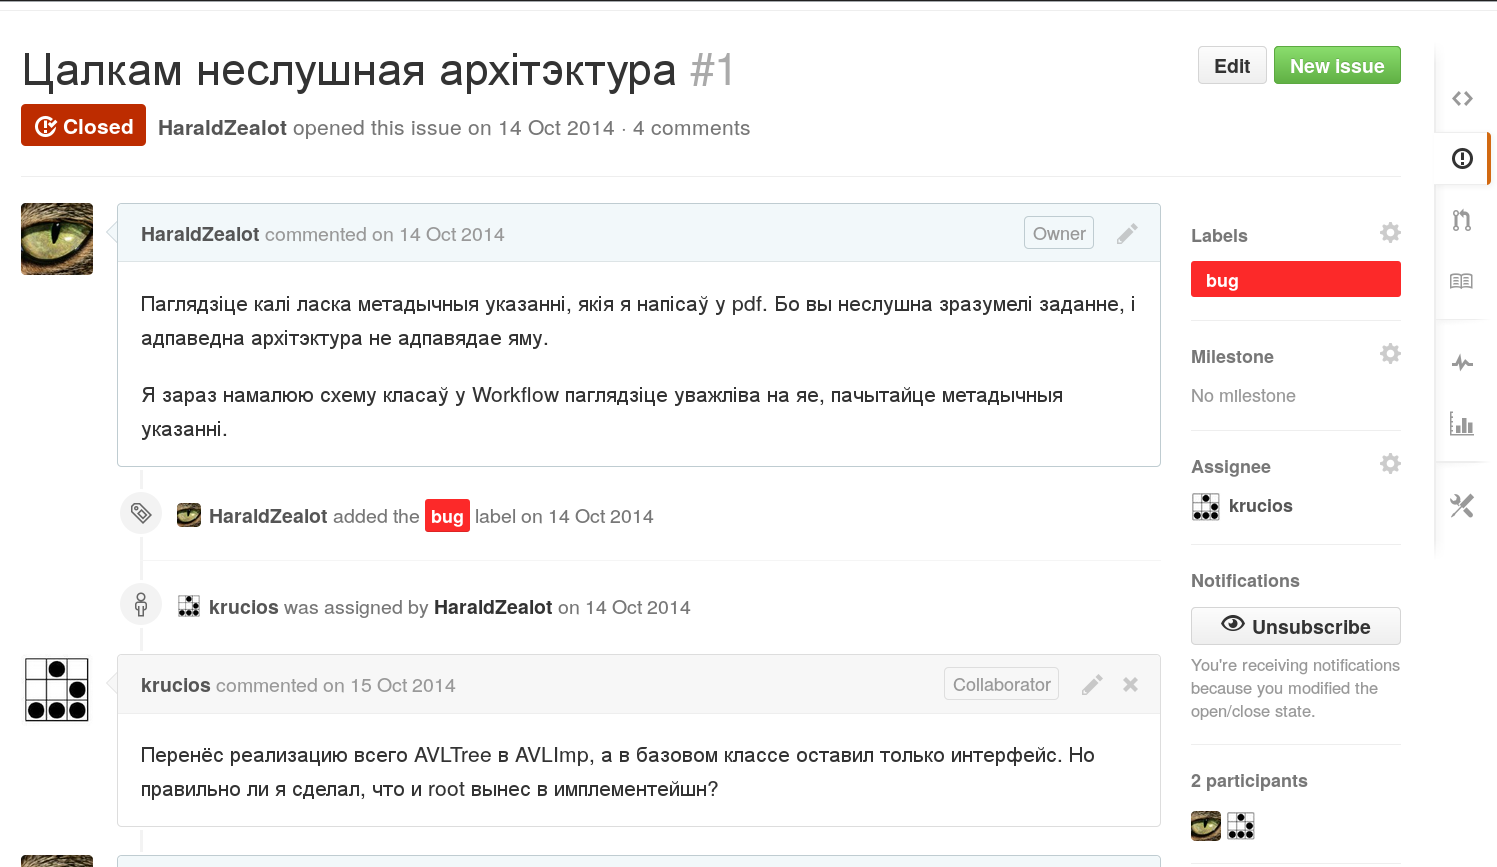
\includegraphics[scale=0.4,keepaspectratio]{snp42.png}
\end{center}
\end{frame}

\begin{frame}{Режим blame; Курсовая работа}
\begin{center}
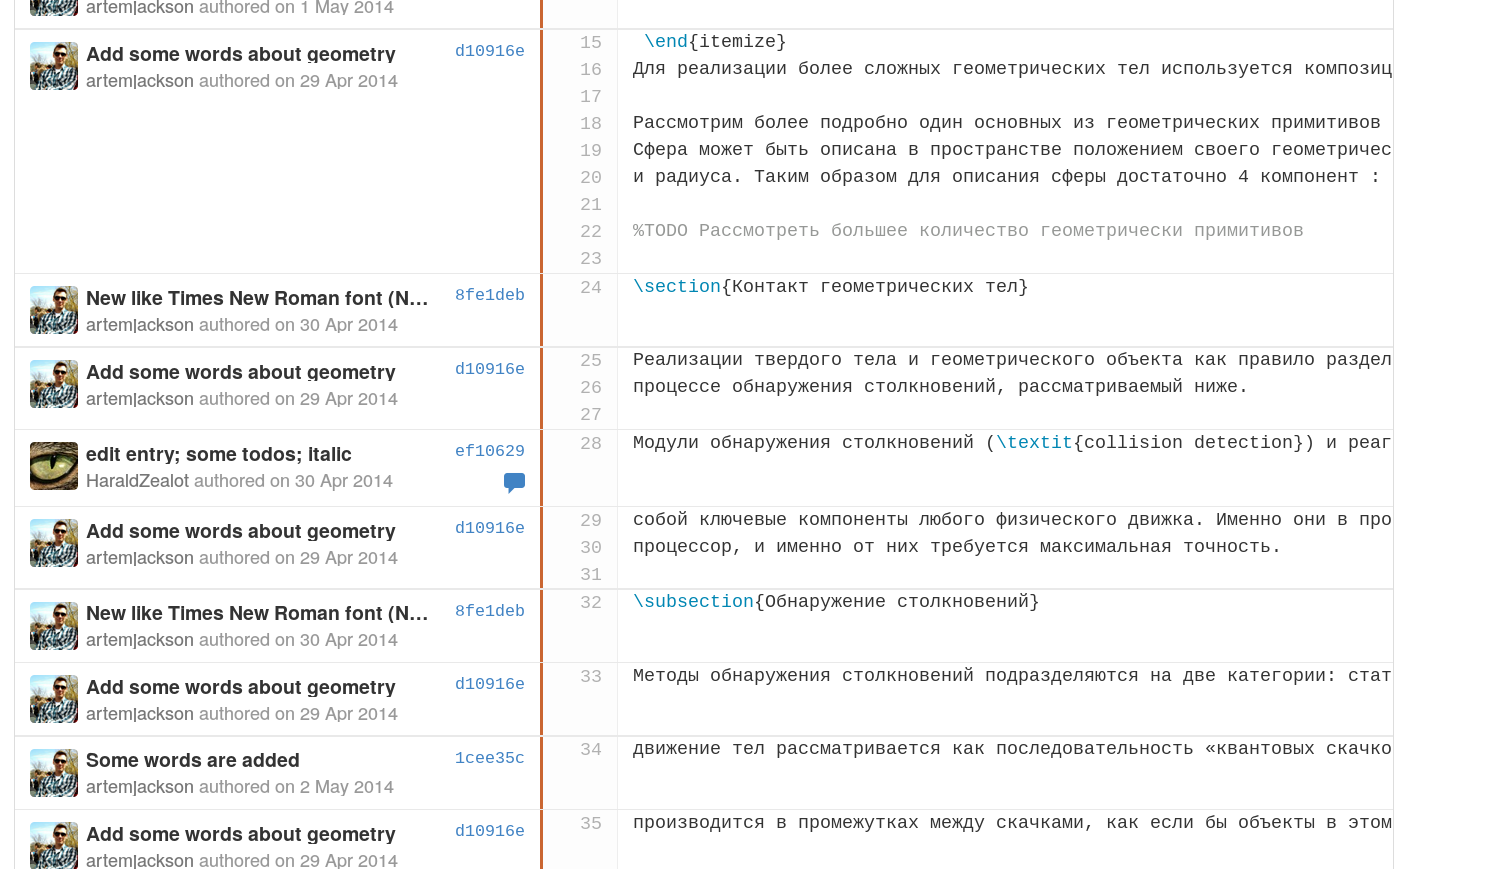
\includegraphics[scale=0.4,keepaspectratio]{snp45.png}
\end{center}
\end{frame}

\begin{frame}{Just for fun}
\begin{center}
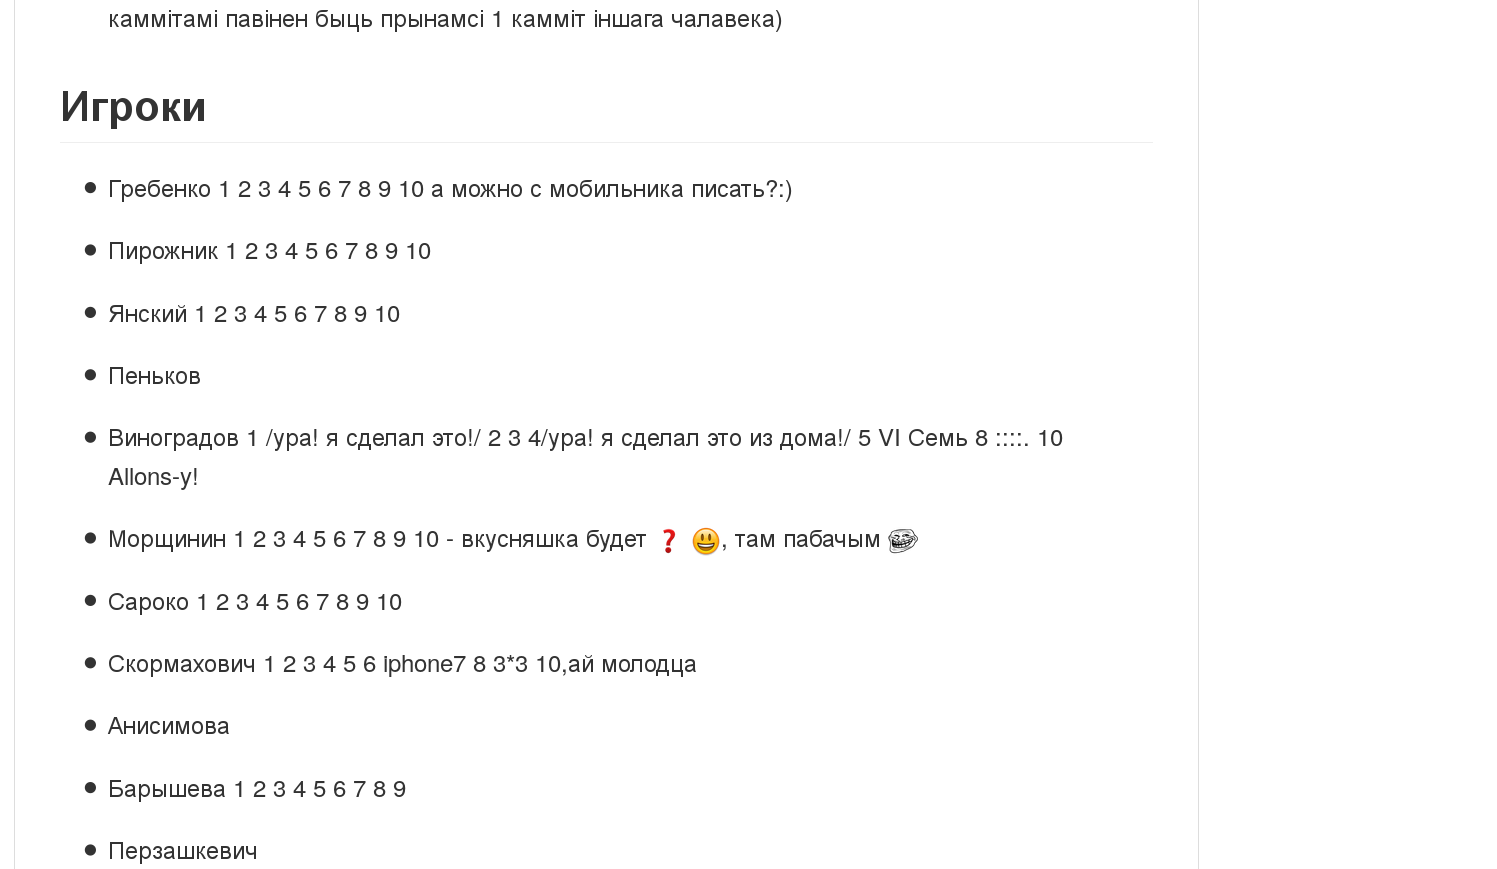
\includegraphics[scale=0.4,keepaspectratio]{snp43.png}
\end{center}
\end{frame}

\begin{frame}{Визуализация веток}
\begin{center}
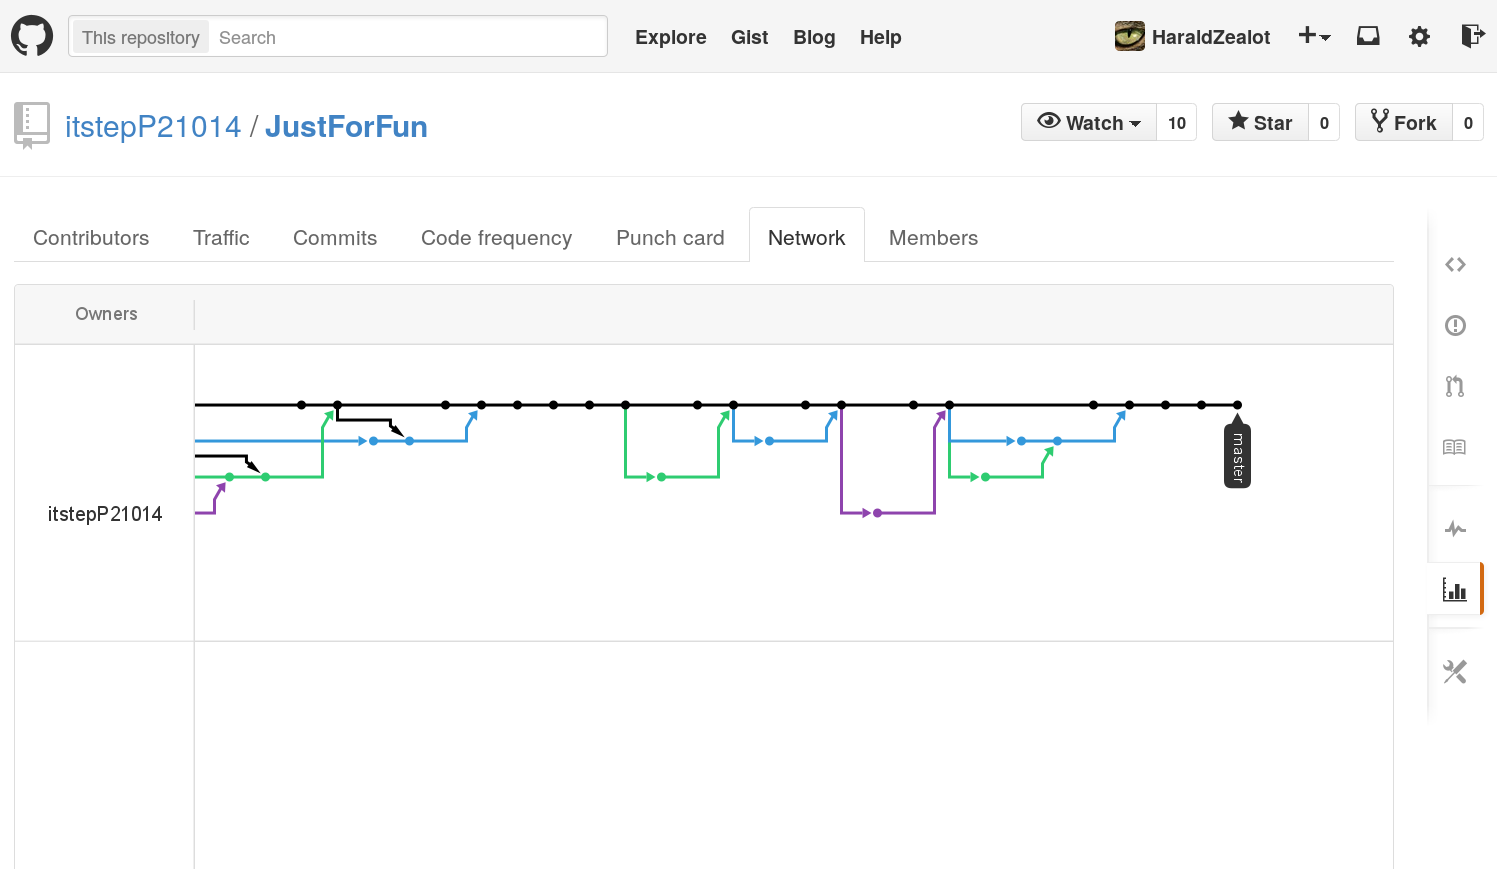
\includegraphics[scale=0.4,keepaspectratio]{snp44.png}
\end{center}
\end{frame}


\end{document}



